\documentclass[final]{article}

\PassOptionsToPackage{numbers,sort&compress}{natbib}
\usepackage{APS360}
\usepackage[utf8]{inputenc}
\usepackage[T1]{fontenc}
\usepackage{hyperref}
\usepackage{url}
\usepackage{booktabs}
\usepackage{amsfonts}
\usepackage{amsmath}
\usepackage{microtype}
\usepackage{xcolor}
\usepackage{graphicx}
\usepackage{array}
\graphicspath{{figures/}{../docs/figures/}}
\makeatletter\providecommand{\@trackname}{}\makeatother
\renewcommand{\bibfont}{\fontsize{8}{9.2}\selectfont}
\setlength{\bibsep}{1.5pt}
\setlength{\intextsep}{2pt}
\setlength{\textfloatsep}{6pt}
\setlength{\abovecaptionskip}{2pt}
\setlength{\belowcaptionskip}{0pt}
\let\oldsection\section
\renewcommand{\section}{\vspace{-0.4em}\oldsection}
\let\oldsubsection\subsection
\renewcommand{\subsection}{\vspace{-0.4em}\oldsubsection}
% The e-mail is kept out of the public repository: progress_report/author_private.tex (gitignored)
% holds \renewcommand{\authoremail}{, <email>} for the submitted build.
\newcommand{\authoremail}{}
\IfFileExists{author_private.tex}{\input{author_private.tex}}{}

\title{The Shape of a Knowledge Boundary: Progress Report\\
A Transformer Trained Only on Pre-1939 Text}

\author{%
  Andrew An \\
  1010864165\authoremail\\
  \url{https://github.com/Shinoaki798/1939}\\
  I used Claude to write the code and draft this report.\\
}

\raggedbottom
\begin{document}

\maketitle

\vspace{-0.42in}

\section*{Brief Project Description}
A language model's knowledge cutoff is usually described as a wall. This project asks what it really looks like.
I train a \textbf{decoder-only Transformer from random initialisation only on text published up to 30 June 1939}
--- American newspapers, and German newspapers in the original --- and measure where and how its knowledge ends.
\textbf{Input:} a sequence of tokens of period text. \textbf{Output:} a probability for every possible next token
(Figure~\ref{fig:overview}). Every measurement comes from that one output: bits per byte (bpb) on held-out articles
of each year 1900--1955 shows where knowledge ends; a forced choice between candidate answers shows what the model
knows about 1939 and which post-1939 concepts it can reach (RQ1) or foresee (RQ3); a fine-tuned copy answers
questions in the newspapers' own question-column format. This matters because every deployed language model has a
cutoff, but none has one that is hard and verifiable: here no text after the cutoff exists in training, so the
boundary can be measured without contamination. \textbf{Why deep learning:} the quantities exist only as the
next-token distribution of a model trained on the text. Count-based models give probabilities only for what they have
seen (the $n$-gram baseline is the floor); a neural language model generalises to unseen articles and
questions. \textbf{Changes since the proposal:} German is used in the original (no translation); the English-only twin
for RQ2 was dropped by its pre-registered criterion (below); fine-tuning a copy was added.

\begin{figure}[!h]
  \centering
  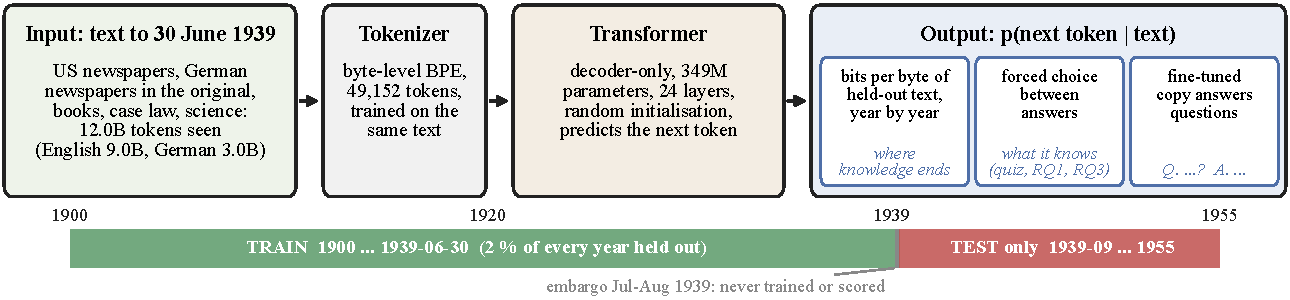
\includegraphics[width=\textwidth]{overview.pdf}
  \vspace{-1.4em}
  \caption{Input, model and output, and the split by publication date.}
  \label{fig:overview}
\end{figure}

\section*{Notable Contribution}
\subsection*{Data Processing}
\textbf{Sources} (all public domain or openly licensed, dated, pre-cutoff): \emph{English} --- American Stories
\citep{dell2023} (article-level text from Chronicling America; the only source of scored sets), Chronicling America
page OCR for the 1930s \citep{chronam2026}, the Congressional Record \citep{gentzkow2018}, case law
\citep{cap2024}, public-domain books \citep{locpdbooks}; \emph{German} --- Europeana \citep{europeana2015} and
Deutsches Zeitungsportal \citep{ddb2024} newspapers, \emph{V\"olkischer Beobachter} \citep{vb1925}; \emph{science}
--- JSTOR \citep{jstorejc}, \emph{Nature}, \emph{Annalen der Physik} \citep{iascience}, JFM reviews \citep{jfm}.
\textbf{Steps} (code \texttt{src/data/}, each stage content-addressed with a manifest):
(1)~ingest one row per article, page or book with its date; (2)~language vote on stopwords; (3)~OCR score per
document: share of words in a period lexicon and share of word-like tokens; (4)~MinHash near-duplicate removal on the
pooled selection (word 5-grams, 128 permutations, LSH $32\times4$, keep the earliest copy; English: 3.66M of 65.7M
documents dropped); (5)~split by date, never shuffled: a fixed 2\,\% of every year 1900--1955 per language held out
\emph{before} OCR filtering, Val a disjoint 2\,\% $\le$ cutoff, 1939-07-01\,...\,08-31 set aside as an embargo; (6)~remove
training paragraphs that also occur in held-out articles (16M words) and wire-service reprints (EN 150M, DE 155M
words); (7)~OCR gates (lexicon share $\ge$ 0.75, word-like $\ge$ 0.70, $\ge$ 50 tokens), long documents cut into
chunks; (8)~mixture: 1934--39 text seen twice, everything else at most once, recency weight
$\propto e^{-(1939-\text{year})/5}$ within a period, German $\le$ 25\,\%, books $\le$ 12\,\%, law $\le$ 10\,\%;
(9)~byte-level BPE with 49,152 tokens trained on the same text; documents in a seeded hash order, an end-of-text token
after each, cut into rows of 4,096 tokens. Table~\ref{tab:data} gives the result.

\begin{table}[!h]
\vspace{2pt}
\centering\footnotesize\setlength{\tabcolsep}{4pt}
\caption{Cleaned data. Left: tokens seen in training. Right: held-out American Stories sets (never trained on).}
\label{tab:data}
\begin{tabular}{@{}lrrr@{}}
\toprule
period & English & German & total \\
\midrule
1930--1939.06 & 5.53B & 1.84B & 7.37B \\
1920--1929 & 2.01B & 0.67B & 2.68B \\
1900--1919 & 0.61B & 0.19B & 0.80B \\
science (any year) & 0.85B & 0.30B & 1.15B \\
\midrule
total (23.7M documents) & 9.00B & 3.00B & \textbf{12.00B} \\
\bottomrule
\end{tabular}\hfill
\begin{tabular}{@{}lrr@{}}
\toprule
set & articles & words \\
\midrule
Val, $\le$ 1939-06-30 & 931,573 & 137.5M \\
Test-A, 1930--38 & 181,156 & 27.1M \\
Test-B, 1939-09--1945 & 124,858 & 18.0M \\
Test-C, 1946--55 & 120,602 & 18.3M \\
per-year bpb set, 1900--55 & 222,843 & 51.9M tok. \\
\bottomrule
\end{tabular}
\vspace{2pt}
\end{table}

\noindent\textbf{A cleaned training sample} (American Stories, 1939-04-11, OCR score 0.98, excerpt; remaining OCR
errors kept as they are): \emph{``The main issues Of the campaign are probably included in this list of ten: (D
Diversion Of highway funds; (2) homestead exemption; CD teach er retirement; (4) extension of ad valorem taxes for
State purposes; \ldots''}
\textbf{Testing on never-seen data.} No text dated after 1939-06-30 is in training, so every article from 1939-09 to
1955 (Test-B, Test-C) is new to the model, and the 2\,\% held out per year was set aside before OCR filtering.
New test sets I write myself are frozen by checksum before any model sees them: a 121-item quiz on the news of 1939
(done), the RQ1 probe set and the RQ3 propositions. An entirely different dataset, ChroniclingAmericaQA
\citep{piryani2024}, tests the fine-tuned copy.
\textbf{Challenges:} OCR noise (99\,\% of the German-language American Stories articles, Fraktur read as Latin script, fail the gates); wire stories
printed in hundreds of papers; very uneven supply (1920--22 has 1.1--1.2B words a year, 1925--29 about 0.25B); and
scale on one machine (the WSL disk grew to 888\,GB before the intermediate files were deleted at the corpus freeze).

\subsection*{Baseline Model}
Three recurrent language models --- a \textbf{vanilla RNN} (tanh), an \textbf{LSTM} and a \textbf{GRU}: token embedding,
2 recurrent layers, output layer tied to the embedding, softmax over 49,152 tokens, $\approx$50M parameters each --- trained
on exactly the same 12B-token stream, tokenizer and schedule as the Transformer (45,776 steps of $2^{18}$ tokens, AdamW,
1,000 warm-up steps, cosine decay, rows of 4,096 tokens with the state reset per row), plus a \textbf{Kneser--Ney
5-gram} (KenLM, first 1B tokens) as the non-neural floor. The learning rate was picked from 200M-token probes of
$\{5\text{e-}4, 1\text{e-}3, 2\text{e-}3\}$ by Val bpb, the RNN's grid extended downwards. Each recurrent run took
17.6\,h on the RTX~5080. All models are scored on the same held-out documents in bits per byte.
\textbf{Quantitative} (Table~\ref{tab:models}, Figure~\ref{fig:results}): the GRU is the best baseline (Val English
1.526 bpb), and every model is worse on articles written after the cutoff than before it.
\textbf{Qualitative:} given \emph{``who is Hitler''}, the GRU continues ``\emph{'s new minister, and who is now in the
midst of the great war, is the first to be elected. The first of the new members of the cabinet is the new president,
DR.. William H. King} \ldots'' --- fluent locally, no persistent subject. \textbf{Challenges:} the LSTM at
$1\text{e-}3$ and the RNN above $5\text{e-}4$ stalled at the unigram plateau; one GRU run survived a 1.9\,h power
loss by resuming exactly from its checkpoint.

\begin{table}[!h]
\vspace{2pt}
\centering\footnotesize\setlength{\tabcolsep}{4pt}
\caption{All models on the same data. After/before: mean English bpb of held-out articles 1940--55 over 1930--38.}
\label{tab:models}
\begin{tabular}{@{}lllllr@{}}
\toprule
model & layers $\times$ width & parameters & learning rate & Val English bpb & after/before \\
\midrule
Kneser--Ney 5-gram & order 5 & 1.7B $n$-grams & --- & --- & $+14.4\,\%$ \\
RNN (tanh) & $2\times960$ & 50.9M & $2.5\times10^{-4}$ & 1.711 & $+11.1\,\%$ \\
LSTM & $2\times800$ & 49.6M & $2\times10^{-3}$ & 1.545 & $+12.9\,\%$ \\
GRU & $2\times832$ & 49.2M & $2\times10^{-3}$ & 1.526 & $+13.5\,\%$ \\
\textbf{Transformer (primary)} & $24\times1{,}024$ & 349.2M & $3\times10^{-4}$ & \textbf{1.181} [1.176, 1.186] &
$+19.4\,\%$ \\
\bottomrule
\end{tabular}
\vspace{2pt}
\end{table}

\begin{figure}[!h]
  \centering
  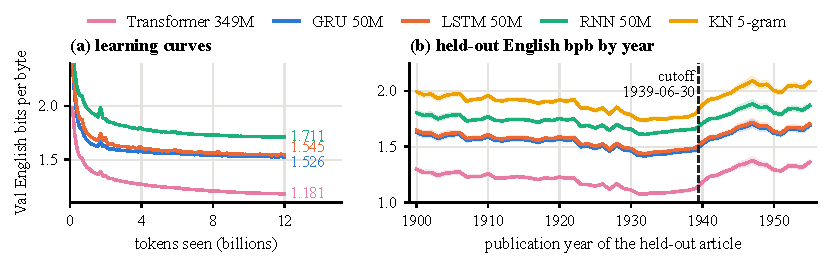
\includegraphics[width=\textwidth]{results.pdf}
  \vspace{-1.6em}
  \caption{(a) Val English bpb during training; all four networks read the same stream. (b) English bpb of held-out
  articles by publication year, bands = bootstrap 95\,\% CI over documents.}
  \label{fig:results}
\end{figure}

\subsection*{Primary Model}
\begin{figure}[!ht]
  \centering
  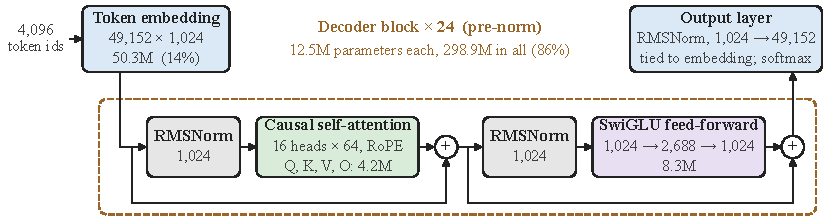
\includegraphics[width=\textwidth]{architecture.pdf}
  \vspace{-1.5em}
  \caption{The primary model, 349,225,984 parameters; each layer with its size.}
  \label{fig:arch}
\end{figure}

\textbf{Architecture and training} (Figure~\ref{fig:arch}; written from scratch in \texttt{src/model/}):
token embedding $49{,}152\times1{,}024$ tied to the output layer; 24 pre-norm decoder blocks, each RMSNorm, causal
self-attention with 16 heads of 64 and rotary position embeddings (base $10^4$), RMSNorm, SwiGLU feed-forward
$1{,}024\to2{,}688\to1{,}024$, residual connections; context 4,096. Next-token cross-entropy, AdamW
($\beta=0.9, 0.95$, weight decay 0.1), peak learning rate $3\times10^{-4}$, 1,000 warm-up steps, cosine to 10\,\%,
gradient clipping 1.0, bf16, 64 rows of 4,096 per step (262,144 tokens), 45,776 steps $=$ 12.0B tokens, seed 1939.
117\,h (4.9 days) on one RTX~5080 (16\,GB), a checkpoint every 500 steps; a resume test passed before launch.
\textbf{Quantitative} (95\,\% CI): Val English \textbf{1.181} [1.176, 1.186] bpb, 23\,\% below the best baseline
(GRU 1.526); German 1.565 [1.519, 1.612]. Per year (Figure~\ref{fig:results}b) bpb falls to 1.075 in 1932, rises
slowly to 1.125 in 1939 and then faster (1.182 in 1940, 1.378 in 1947): mean 1940--55 is $+19.4\,\%$ over 1930--38,
the largest relative rise of all models (Table~\ref{tab:models}). It is a ramp that steepens at the cutoff rather
than a clean step; the OCR-quality covariate is still to be regressed out. \textbf{Cross-lingual check} (decides the
RQ2 twin, criterion fixed in advance): a German article on the same topic makes an English passage \emph{less} likely
than one on another topic ($-0.021$ [$-0.030$, $-0.013$] bpb), while an English article on the same topic helps
($+0.021$ [0.009, 0.033]); so no twin is trained, and RQ2 is answered from this check.
\textbf{1939 news quiz} (121 four-choice items written and frozen first; chance 25\,\%): 39\,\% [30, 48] as a question,
46\,\% [36, 55] as a statement on the 101 pre-cutoff items; 31--35\,\% on the last year before the cutoff; 15\,\% on
post-cutoff controls. Wrong answers are often the previous holder of an office (King of England $\to$ Edward VIII,
Poland $\to$ Pilsudski): the model's ``present'' lags behind 1939. The GRU scores the same (40\,\%, 41\,\%), which suggests this
format rewards familiar names more than knowledge.
\textbf{Fine-tuned copy} (answer-only loss on 14,106 period ``Q.\,...?\,A.\,...'' column pairs and 39,162
ChroniclingAmericaQA items, with replay of pretraining text): reading-comprehension exact match on ChroniclingAmericaQA
rises from 1.3\,\% to \textbf{38.8\,\%} [36.7, 41.0] at a cost of $+0.5\,\%$ Val bpb; without replay the cost was
$+4.5\,\%$.

\begin{table}[!h]
\vspace{2pt}
\centering\footnotesize\setlength{\tabcolsep}{4pt}
\caption{Qualitative: greedy answers of the untuned model to questions in the period column format.}
\label{tab:qual}
\begin{tabular}{@{}>{\raggedright\arraybackslash}p{4.6cm}>{\raggedright\arraybackslash}p{5.3cm}>{\raggedright\arraybackslash}p{3.6cm}@{}}
\toprule
question & answer & reading \\
\midrule
Who is the Chancellor of Germany? & Adolf Hitler. & correct \\
What became of Amelia Earhart? & She was lost in the Pacific ocean. & correct (1937) \\
Who is the President of the United States? & Woodrow Wilson. & its ``present'' lags \\
What is a jeep? & A fish that is caught in the sea. & post-1939 sense unknown \\
What happened at Pearl Harbor? & The Navy Department said that [it] had no information as to the cause of the accident. & a naval station, not an attack \\
\bottomrule
\end{tabular}
\vspace{2pt}
\end{table}

\noindent\textbf{Challenges:} the RTX~5080 had blacked out under sustained load, so the 117\,h run was made
resumable and checked every two hours (it finished without a crash); the first cross-lingual design scored the target
after an end-of-text token, where the model resets, and had to be redone; fine-tuning first cost 4.5\,\% of general
ability until replay was added. \textbf{Feasibility:} all training is finished; what remains --- the OCR covariate,
building and freezing the RQ1 probe set ($\sim$200 terms) and the RQ3 propositions ($\ge$120), the
ChroniclingAmericaQA sanity check on the untuned model, the final report --- is evaluation only, each scoring run under
an hour on the 5080, scheduled 20 Nov\,--\,6 Dec.

\newpage
\bibliographystyle{abbrvnat}
\bibliography{../docs/references}

\end{document}
